\documentclass[journal, a4paper]{IEEEtran}

% some very useful LaTeX packages include:

%\usepackage{cite}      % Written by Donald Arseneau
                        % V1.6 and later of IEEEtran pre-defines the format
                        % of the cite.sty package \cite{} output to follow
                        % that of IEEE. Loading the cite package will
                        % result in citation numbers being automatically
                        % sorted and properly "ranged". i.e.,
                        % [1], [9], [2], [7], [5], [6]
                        % (without using cite.sty)
                        % will become:
                        % [1], [2], [5]--[7], [9] (using cite.sty)
                        % cite.sty's \cite will automatically add leading
                        % space, if needed. Use cite.sty's noadjust option
                        % (cite.sty V3.8 and later) if you want to turn this
                        % off. cite.sty is already installed on most LaTeX
                        % systems. The latest version can be obtained at:
                        % http://www.ctan.org/tex-archive/macros/latex/contrib/supported/cite/

\usepackage{graphicx}   % Written by David Carlisle and Sebastian Rahtz
                        % Required if you want graphics, photos, etc.
                        % graphicx.sty is already installed on most LaTeX
                        % systems. The latest version and documentation can
                        % be obtained at:
                        % http://www.ctan.org/tex-archive/macros/latex/required/graphics/
                        % Another good source of documentation is "Using
                        % Imported Graphics in LaTeX2e" by Keith Reckdahl
                        % which can be found as esplatex.ps and epslatex.pdf
                        % at: http://www.ctan.org/tex-archive/info/

%\usepackage{psfrag}    % Written by Craig Barratt, Michael C. Grant,
                        % and David Carlisle
                        % This package allows you to substitute LaTeX
                        % commands for text in imported EPS graphic files.
                        % In this way, LaTeX symbols can be placed into
                        % graphics that have been generated by other
                        % applications. You must use latex->dvips->ps2pdf
                        % workflow (not direct pdf output from pdflatex) if
                        % you wish to use this capability because it works
                        % via some PostScript tricks. Alternatively, the
                        % graphics could be processed as separate files via
                        % psfrag and dvips, then converted to PDF for
                        % inclusion in the main file which uses pdflatex.
                        % Docs are in "The PSfrag System" by Michael C. Grant
                        % and David Carlisle. There is also some information
                        % about using psfrag in "Using Imported Graphics in
                        % LaTeX2e" by Keith Reckdahl which documents the
                        % graphicx package (see above). The psfrag package
                        % and documentation can be obtained at:
                        % http://www.ctan.org/tex-archive/macros/latex/contrib/supported/psfrag/

%\usepackage{subfigure} % Written by Steven Douglas Cochran
                        % This package makes it easy to put subfigures
                        % in your figures. i.e., "figure 1a and 1b"
                        % Docs are in "Using Imported Graphics in LaTeX2e"
                        % by Keith Reckdahl which also documents the graphicx
                        % package (see above). subfigure.sty is already
                        % installed on most LaTeX systems. The latest version
                        % and documentation can be obtained at:
                        % http://www.ctan.org/tex-archive/macros/latex/contrib/supported/subfigure/

\usepackage{url}        % Written by Donald Arseneau
                        % Provides better support for handling and breaking
                        % URLs. url.sty is already installed on most LaTeX
                        % systems. The latest version can be obtained at:
                        % http://www.ctan.org/tex-archive/macros/latex/contrib/other/misc/
                        % Read the url.sty source comments for usage information.

%\usepackage{stfloats}  % Written by Sigitas Tolusis
                        % Gives LaTeX2e the ability to do double column
                        % floats at the bottom of the page as well as the top.
                        % (e.g., "\begin{figure*}[!b]" is not normally
                        % possible in LaTeX2e). This is an invasive package
                        % which rewrites many portions of the LaTeX2e output
                        % routines. It may not work with other packages that
                        % modify the LaTeX2e output routine and/or with other
                        % versions of LaTeX. The latest version and
                        % documentation can be obtained at:
                        % http://www.ctan.org/tex-archive/macros/latex/contrib/supported/sttools/
                        % Documentation is contained in the stfloats.sty
                        % comments as well as in the presfull.pdf file.
                        % Do not use the stfloats baselinefloat ability as
                        % IEEE does not allow \baselineskip to stretch.
                        % Authors submitting work to the IEEE should note
                        % that IEEE rarely uses double column equations and
                        % that authors should try to avoid such use.
                        % Do not be tempted to use the cuted.sty or
                        % midfloat.sty package (by the same author) as IEEE
                        % does not format its papers in such ways.

\usepackage{amsmath}    % From the American Mathematical Society
                        % A popular package that provides many helpful commands
                        % for dealing with mathematics. Note that the AMSmath
                        % package sets \interdisplaylinepenalty to 10000 thus
                        % preventing page breaks from occurring within multiline
                        % equations. Use:
%\interdisplaylinepenalty=2500
                        % after loading amsmath to restore such page breaks
                        % as IEEEtran.cls normally does. amsmath.sty is already
                        % installed on most LaTeX systems. The latest version
                        % and documentation can be obtained at:
                        % http://www.ctan.org/tex-archive/macros/latex/required/amslatex/math/
\usepackage{bm}
\usepackage{algorithm}
\usepackage{algorithmic}
\usepackage{setspace}
% \usepackage{algorithm2e}


% Other popular packages for formatting tables and equations include:

%\usepackage{array}
% Frank Mittelbach's and David Carlisle's array.sty which improves the
% LaTeX2e array and tabular environments to provide better appearances and
% additional user controls. array.sty is already installed on most systems.
% The latest version and documentation can be obtained at:
% http://www.ctan.org/tex-archive/macros/latex/required/tools/

% V1.6 of IEEEtran contains the IEEEeqnarray family of commands that can
% be used to generate multiline equations as well as matrices, tables, etc.

% Also of notable interest:
% Scott Pakin's eqparbox package for creating (automatically sized) equal
% width boxes. Available:
% http://www.ctan.org/tex-archive/macros/latex/contrib/supported/eqparbox/

% *** Do not adjust lengths that control margins, column widths, etc. ***
% *** Do not use packages that alter fonts (such as pslatex).         ***
% There should be no need to do such things with IEEEtran.cls V1.6 and later.


% Your document starts here!
\begin{document}
\begin{titlepage}

\newcommand{\HRule}{\rule{\linewidth}{0.5mm}} % Defines a new command for the horizontal lines, change thickness here

\center % Center everything on the page
 %----------------------------------------------------------------------------------------
%	LOGO SECTION
%----------------------------------------------------------------------------------------

~\\[1cm]

\includegraphics{SCUT.png}\\[2cm] % Include a department/university logo - this will require the graphicx package

%----------------------------------------------------------------------------------------
%	TITLE SECTION
%----------------------------------------------------------------------------------------

\HRule \\[1cm]
{ \huge \bfseries The Experiment Report of \textit{Machine Learning} }\\[0.6cm] % Title of your document
\HRule \\[2cm]
%----------------------------------------------------------------------------------------
%	HEADING SECTIONS
%----------------------------------------------------------------------------------------


\textsc{\LARGE \textbf{School:} School of Software Engineering}\\[1cm]
\textsc{\LARGE \textbf{Subject:} Software Engineering}\\[2cm]


%----------------------------------------------------------------------------------------
%	AUTHOR SECTION
%----------------------------------------------------------------------------------------

\begin{minipage}{0.4\textwidth}
\begin{flushleft} \large
\emph{Author:}\\
Yawen Xu % Your name
\end{flushleft}
\end{minipage}
~
\begin{minipage}{0.4\textwidth}
\begin{flushright} \large
\emph{Supervisor:} \\
Mingkui Tan % Supervisor's Name
\end{flushright}
\end{minipage}\\[2cm]
~
\begin{minipage}{0.4\textwidth}
\begin{flushleft} \large
\emph{Student ID:}\\
201820137853
\end{flushleft}
\end{minipage}
~
\begin{minipage}{0.4\textwidth}
\begin{flushright} \large
\emph{Grade:} \\
Graduate
\end{flushright}
\end{minipage}\\[2cm]

% If you don't want a supervisor, uncomment the two lines below and remove the section above
%\Large \emph{Author:}\\
%John \textsc{Smith}\\[3cm] % Your name

%----------------------------------------------------------------------------------------
%	DATE SECTION
%----------------------------------------------------------------------------------------

{\large \today}\\[2cm] % Date, change the \today to a set date if you want to be precise


%----------------------------------------------------------------------------------------

\vfill % Fill the rest of the page with whitespace

\end{titlepage}

% Define document title and author
	\title{Logistic Regression and Support Vector Machine}
	\maketitle

% Write abstract here
\begin{abstract}
This project uses logistic regression and support vector machine to solve classification problem. Batch random stochastic gradient descent and Adam are used to optimize the parameters in the two algorithms.
\end{abstract}

% Each section begins with a \section{title} command
\section{Introduction}
	% \PARstart{}{} creates a tall first letter for this first paragraph
\IEEEPARstart{C}{lassification} problem is an important issue in machine learning. Given input variable $X$ and output variable $Y$,  $Y$ is finite and discrete. If a model can predict $Y$ from $X$, we call this model a classification model. If $Y$ only has two values, this classification problem is a binary classification problem.

This experiment implements a logistic regression model and a support vector machine model for binary classification problem. Logistic regression is a kind of log-linear model. Its main idea is relating the true label $y$ to the real value predicted by linear regression with a monotonous and differentiable sigmoid function. Support vector machine is a linear classifier with the largest margin in the feature space, which transforms the classification problem into a convex quadratic programming problem.

This experiment uses stochastic batch gradient descent and Adam method to optimize parameters. The motivation of this experiment is to
\begin{itemize}
  \item compare and understand the differences between gradient descent and batch random stochastic gradient descent;
  \item compare and under the differences and relationships between Logistic regre.ssion and linear classification;
  \item further understand the principles of SVM and practice on larger data;
\end{itemize}

The experimental results on the \textbf{a9a} dataset show that two models both have a good classification performance.


% Main Part
\section{Methods and Theory}

\subsection{Logistic Regression}
Logistic regression is a kind of log-linear model. Its main idea is relating the true label $y$ to the real value predicted by linear regression with a monotonous and differentiable \textbf{sigmoid} function. The \textbf{sigmoid} function is defined as follow:
\begin{equation}
g(z) = \frac{1}{1+e^{-z}}
\end{equation}
where $z \in R$. The function is a continuous function, if $z \rightarrow \infty$, then $g(z) \rightarrow 1$; if $z \rightarrow -\infty$, then $g(z) \rightarrow 0$. In linear regression, the predicted real values is:
\begin{equation}
z = \bm{w}^{T}\bm{x}
\end{equation}
where $\bm{w}$ represents the weights of feature $\bm{x}$. The logistic regression function is defined as follows:
\begin{equation}
h_{\bm{w}}(\bm{x}) = g(\bm{w}^{T}\bm{x}) = \frac{1}{1+e^{-\bm{w}^{T}\bm{x}}}
\end{equation}
The output of $h_{\bm{w}}(\bm{x})$ is a float number in $(0,1)$, which indicates a probability of the occurrence of y. Assume the labels $y_i \in \{-1,+1\}$, we need to find a good h, when $y=1$, $h_{\bm{w}}(\bm{x}) \approx 1$, when $y=-1$, $h_{\bm{w}}(\bm{x}) \approx 0$. Based on that intuitive probabilistic interpretation of $h$, we have a loss function which measures the "goodness" of a logistic regression model:
\begin{equation}
J(\bm{w}) = \frac{1}{n}\sum_{i=1}^{n} log(1+e^{-y_i \cdot \bm{w}^Tx_i}) + \frac{\lambda}{2}\parallel \bm{w} \parallel_2^2
\end{equation}
where $n$ is the number of training samples, $\lambda$ is the regularization term. The gradient of loss with respect to parameters $\frac{\partial J(\bm{w})}{\partial w}$ is:
\begin{equation}
\frac{\partial J(\bm{w})}{\partial \bm{w}} = -\frac{1}{n}\sum_{i=1}^{n}\frac{y_i{\bm{x_i}}}{1+e^{{y_i} \cdot \bm{w}^T\bm{x_i}}}
\end{equation}


When the labels $y_i \in \{0,1\}$, we can derive the loss function in another form:
\begin{equation}
J(\bm{w}) = -\frac{1}{n}[\sum_{i=1}^{n} y_ilogh_{\bm{w}}(\bm{x_i})+(1-y_i)log(1-h_{\bm{w}}(\bm{x_i}))]
\end{equation}

The gradient of loss with respect to parameters $\frac{\partial J(\bm{w})}{\partial w}$ is:
\begin{equation}
\frac{\partial J(\bm{w})}{\partial \bm{w}} = (h_{\bm{w}}(x)-y)\bm{x}
\end{equation}

\subsection{Support Vector Machine}
Support vector machine is a linear classifier with the largest margin in the feature space, which transforms the classification problem into a convex quadratic programming problem. We select two parallel hyperplanes that separate the two classes of data in the feature space, and let the distance between them as large as possible. The region bounded by these hyperplanes is called the ``margin''. SVM aims to find the maximum margin, which is most stable under perturbations of the inputs.

If we choose normalization such that $\bm{w}^{T}\bm{x}_{+} + b = +1$ and $\bm{w}^{T}\bm{x}_{-} + b = -1$ for the positive and negative support vectors respectively, then the margin is given by:
\begin{equation}
  \frac{\bm{w}}{\parallel \bm{w} \parallel}\cdot(\bm{x}_{+}-\bm{x}_{-}) = \frac{\bm{w}^{T}(\bm{x}_{+}-\bm{x}_{-})}{\parallel \bm{w} \parallel} = \frac{2}{\parallel \bm{w} \parallel}
\end{equation}

Learning the SVM can be formulated as an optimization:
\begin{equation}
\max\limits_{\bm{w},b}\frac{2}{\parallel \bm{w} \parallel} \\
s.t.\ \bm{w}^T\bm{x_i}+b
\left\{
             \begin{array}{lr}
             \ge 1, &  y_i = +1\\
             \le 1, & y_i = -1\\
             \end{array}
\right.
\end{equation}
Or equivalently:
\begin{equation}
\min\limits_{\bm{w},b}\frac{2}{\parallel \bm{w} \parallel} \\
s.t.\ y_i(\bm{w}^T\bm{x_i}+b)\ge1, i=1,2,...,n
\end{equation}

In general, there is a trade off between the margin and the number of mistakes on the training data. Moreover, the training data may not be linearly separable. So, we introduce $\xi_i \le 0$ as a ``slack variable'', and the optimization problem can be rewrote as:
\begin{equation}
\min\limits_{\bm{w},b}\frac{2}{\parallel \bm{w} \parallel}+C\sum_{i=1}^{n}\xi_i \\
s.t.\ y_i(\bm{w}^T\bm{x_i}+b)\ge1-\xi_i, i=1,2,...,n
\end{equation}
Let $\xi_i$ as hinge loss, the objective function becomes:
\begin{equation}
\min\limits_{\bm{w},b}\frac{2}{\parallel \bm{w} \parallel}+C\sum_{i=1}^{n}max(0,1-y_i(\bm{w}^T\bm{x_i}+b))
\end{equation}

The gradient of loss with respect to parameters $\bm{w}$ and $\bm{b}$ are:
\begin{equation}
g_{\bm{w}}(x_i)=
\left\{
             \begin{array}{lr}
             -y_i\bm{x_i}, &  1-y_i(\bm{w}^T\bm{x_i}+b) \ge 0\\
             0, & 1-y_i(\bm{w}^T\bm{x_i}+b) < 0\\
             \end{array}
\right.
\end{equation}
\begin{equation}
g_{b}(x_i)=
\left\{
             \begin{array}{lr}
             -y_i, &  1-y_i(\bm{w}^T\bm{x_i}+b) \ge 0\\
             0, & 1-y_i(\bm{w}^T\bm{x_i}+b) < 0\\
             \end{array}
\right.
\end{equation}


\subsection{Batch Random stochastic Gradient Descent}
The stochastic gradient descent method chooses one sample randomly for each iteration, it is fast and easy to calculate, but it is easy to fall into the local optimal solution. Mini batch stochastic gradient descent alleviates this problem, rather than pick one sample, it randomly choose one subset $S_k$ for each iteration. The size of $S_k$ is much smaller than the original data size, and it usually be the powers of 2, such as 16, 32.

\subsection{Adam}

Adam is an algorithm for first-order gradient-based optimization of stochastic objective functions, based on adaptive estimates of lower-order moments. The method is straightforward to implement, is computationally efficient, has little memory requirements, is invariant to diagonal rescaling of the gradients, and is well suited for problems that are large in terms of data and/or parameters.

See Algorithm 1 for pseudo-code of our proposed algorithm Adam.

\begin{algorithm}[htb]
\setstretch{1.1} %设置具有指定弹力的橡皮长度(原行宽的1.35倍)
\caption{}
\label{alg:Framwork}
\begin{algorithmic}
\REQUIRE ~~\\
$\alpha$: Stepsize;\\
$\beta_1, \beta_2 \in [0,1)$: Exponential decay rates for the moment estimates;\\
$f(\theta)$:Stochastic objective function with parameters $\theta$;\\
$\theta_0$:Initial parameter vector;\\

$m_0 \leftarrow 0$(Initialize $1^{st}$ moment vector);\\
$v_0 \leftarrow 0$(Initialize $2^{nd}$ moment vector);\\
$t \leftarrow 0$(Initialize timestep);\\
\textbf{while} $\theta_t$ not converged \textbf{do} \\
$t \leftarrow t+1$;\\
$g_t \leftarrow \nabla_\theta f_{t}(\theta_t-1)$(Get gradients w.r.t stochastic objective at timestep t);\\
$m_t \leftarrow \beta_1 \cdot m_{t-1} + (1-\beta_1) \cdot g_t$(Update biased first moment estimate);\\
$v_t \leftarrow \beta_2 \cdot v_{t-1} + (1-\beta_2) \cdot {g_t}^2$(Update biased second raw moment estimate);\\
$\hat{m}_t \leftarrow m_t/(1-\beta_{1}^{t})$(Compute bias-corrected first moment estimate);\\
$\hat{v}_t \leftarrow v_t/(1-\beta_{2}^t)$(Compute bias-corrected second raw moment estimate);\\
$\theta_t \leftarrow \theta_{t-1} - \alpha \cdot \hat{m}_t/(\sqrt(\hat{v_t}) + \epsilon)$(Update parameters);\\
end while\\
return $\theta_t$(Resulting parameters)
\end{algorithmic}
\end{algorithm}

\section{Experiments}
\subsection{Dataset}
 This project uses \textbf{a9a} in \textbf{LIBSVM Data}, including 32561 training samples and 16281 testing samples. Each sample has 123 features. We use the scaled version, which did the feature scaling in the preprocessing step.

\subsection{Implementation}

\begin{itemize}
  \item \textbf{Initialization} We should initialize the parameters before training. In logistic regression experiment, we need to initialize $\bm{w}$. We have three options to initialize it, set $\bm{w}$ into zero, initialize it randomly or with normal distribution. we use these three methods to measure the initialization influence on result.In support vector machine experiment, we need to initialize parameters $\bm{w}$ and $b$. We use the same three methods to initialize $\bm{w}$ and $b$.

      Note that, we have a trade-off parameter $\lambda$ in the logistic regression loss function, and a penalty term $C$ in support vector machine loss function. To see the difference, we set $\lambda$ and $C$ to 0.0, 1.0, 10.0 relatively.
%
  \item \textbf{Training} In LR and SVM, we optimize parameters both in two methods: batch SGD and Adam. We also have some hyperparameters in this experiment, such as batch size $\lvert S_{k}\rvert$, learning rate $\eta$, exponential decay rates $\beta_1$, $\beta_2$ and $\epsilon$. 
      
      We fix $\beta_1=0.9$, $\beta_2=0.999$ and $\epsilon=10^{-8}$. And we adjust the hyperparameters $\lvert S_{k} \rvert$ and $\eta$. We set $\eta$ to 0.1, 0.01 and 0.001, see the influence on result. Then we fix $\eta$, set $|S_{k}|$ to 16, 32, and 64, and see the influence on result.
%
  \item \textbf{Results} In the closed-form solution, we repeat this experiment for five times and test whether the loss will change or not. Fig.~\ref{fig:cf1} shows that the best $\bm{w}$ is unique and the loss will not change.

    % This is how you include a eps figure in your document. LaTeX only accepts EPS or TIFF files.
	\begin{figure}[!hbt]
		% Center the figure.
		\begin{center}
		% Include the eps file, scale it such that it's width equals the column width. You can also put width=8cm for example...
		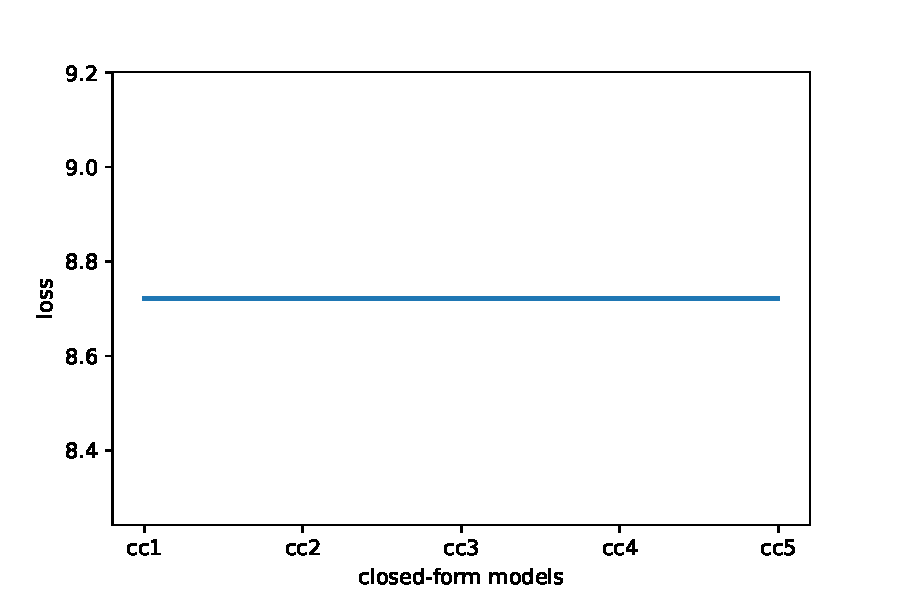
\includegraphics[width=\columnwidth]{cf1}
		% Create a subtitle for the figure.
		\caption{The loss value for five closed-form linear regression models. This figure shows that the best $\bm{w}$ is unique and the loss will not change.}
		% Define the label of the figure. It's good to use 'fig:title', so you know that the label belongs to a figure.
		\label{fig:cf1}
		\end{center}
	\end{figure}


\end{itemize}


\section{Conclusion}
From this project, we have a deeper understanding of linear regression, closed-form solution and stochastic gradient descent. We find that parameters have a large impact on our results, so we should adjust parameters carefully.


% Your document ends here!
\end{document} 